% Section content template for individual Educative lessons
% This file contains the actual content for a specific section
% Generated from Educative API section content

% Section: Requirements for LinkedIn
% Section ID: 6676498603048960
% Section Slug: requirements-for-linkedin
% Generated: 2025-12-14T13:34:08.201806

In this lesson, we'll list the requirements of the LinkedIn design problem. This is a crucial step because requirements define the scope of a problem. Therefore, accurately obtaining and thoroughly understanding them from the interviewer will make the design of the rest of the system smooth and easy.
\\
We'll use the notational convention to identify each requirement with a unique label, ``Rn,'' where ``R'' is short for requirement and ``n'' is a natural number.

\subsection{Requirements collection}\label{O5pF28UFA1P2hHyNNvsGl}
\\
The requirements for LinkedIn are defined below:

% \vspace{-1.0\baselineskip}
\noindent
\begin{minipage}[t]{0.48\textwidth}\vspace{0pt}
\textbf{R1:} Users should be able to add information to their profiles, including education, experiences, achievements, and skills.
\\
\textbf{R2:} Users should be able to search for and view pages, groups, and other users.
\\
\textbf{R3:} Users should be able to send and cancel connection requests and respond to other users' connection requests by either accepting or ignoring them.
\end{minipage}
\hfill
\begin{minipage}[t]{0.48\textwidth}\vspace{0pt}
\centering
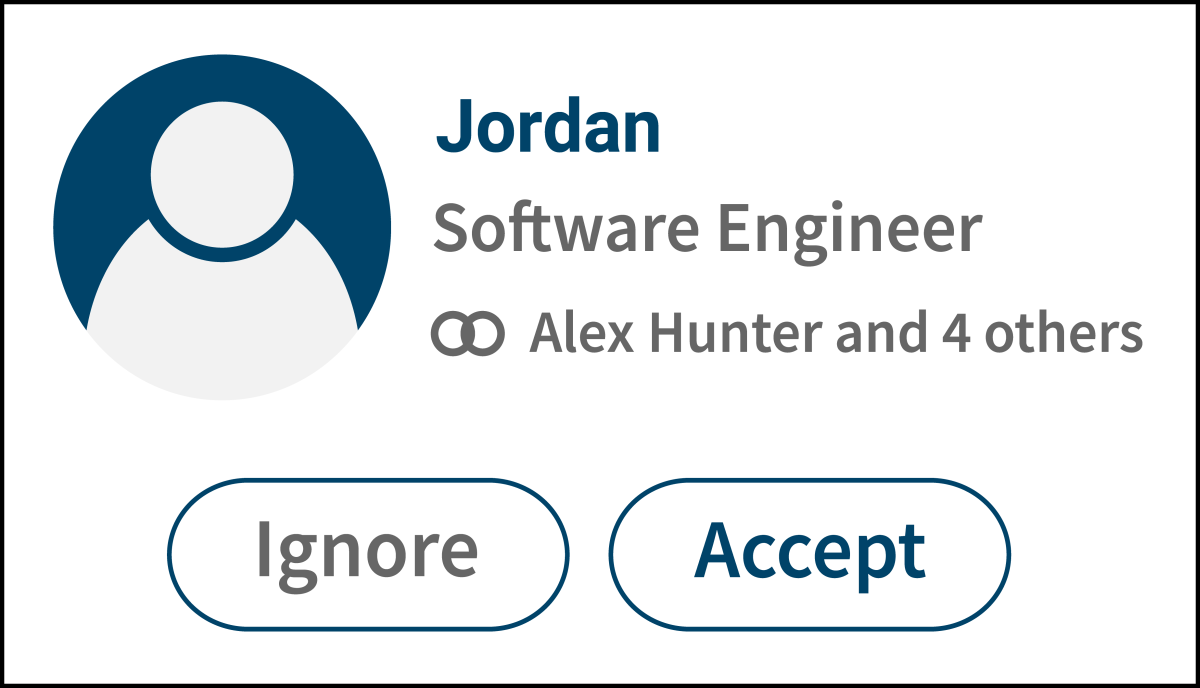
\includegraphics[width=0.5\textwidth]{Images/chapter_27/section_6676498603048960/6160884780236800.png}
\end{minipage}

% \vspace{-1.0\baselineskip}
\noindent
\begin{minipage}[t]{0.48\textwidth}\vspace{0pt}
\textbf{R4:} Users should be able to follow other users without needing to add them as a connection.
\\
\textbf{R5:} Users should be able to view their number of connections, profile views, post impressions, and search appearances.
\\
\textbf{R6:} Users should be able to request and give recommendations to other users.
\end{minipage}
\hfill
\begin{minipage}[t]{0.48\textwidth}\vspace{0pt}
\centering
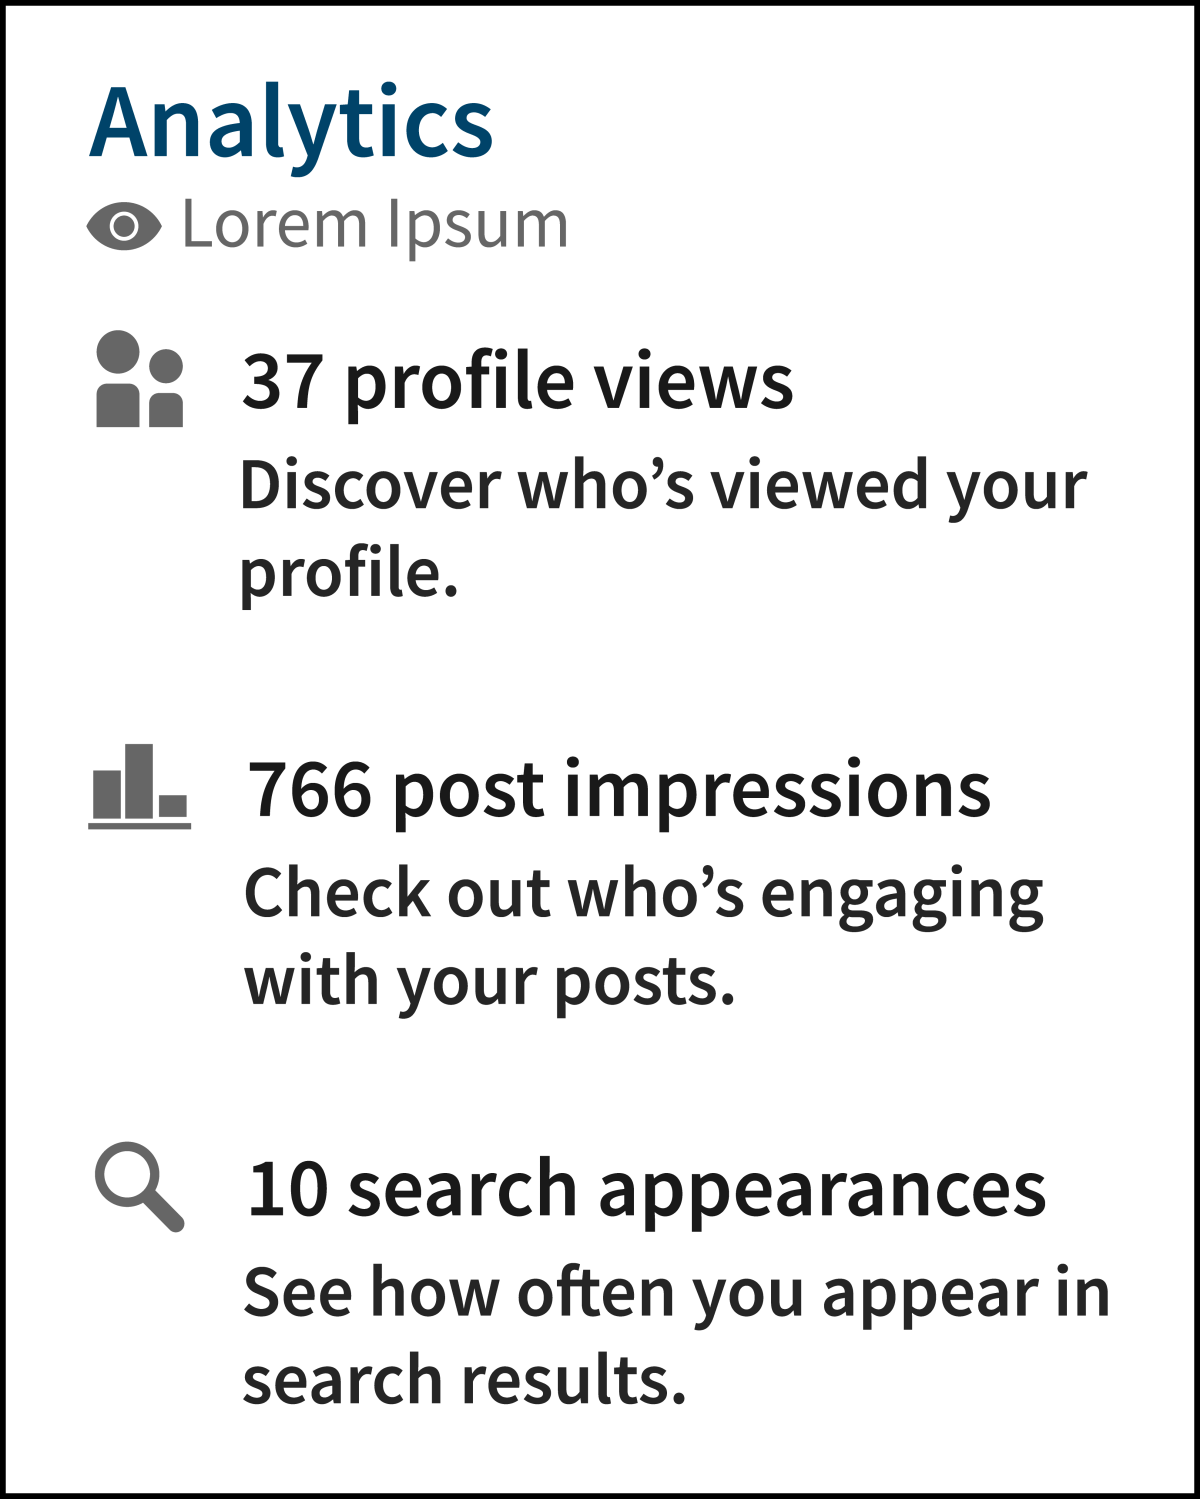
\includegraphics[width=0.5\textwidth]{Images/chapter_27/section_6676498603048960/6199763646283776.png}
\end{minipage}

% \vspace{-1.0\baselineskip}
\noindent
\begin{minipage}[t]{0.48\textwidth}\vspace{0pt}
\textbf{R7:} Users should be able to write a new post.
\\
\textbf{R8:} Users should be able to react, share, and comment on a post and on an existing comment.
\\
\textbf{R9:} A user should be able to send and receive messages from other users.
\end{minipage}
\hfill
\begin{minipage}[t]{0.48\textwidth}\vspace{0pt}
\centering
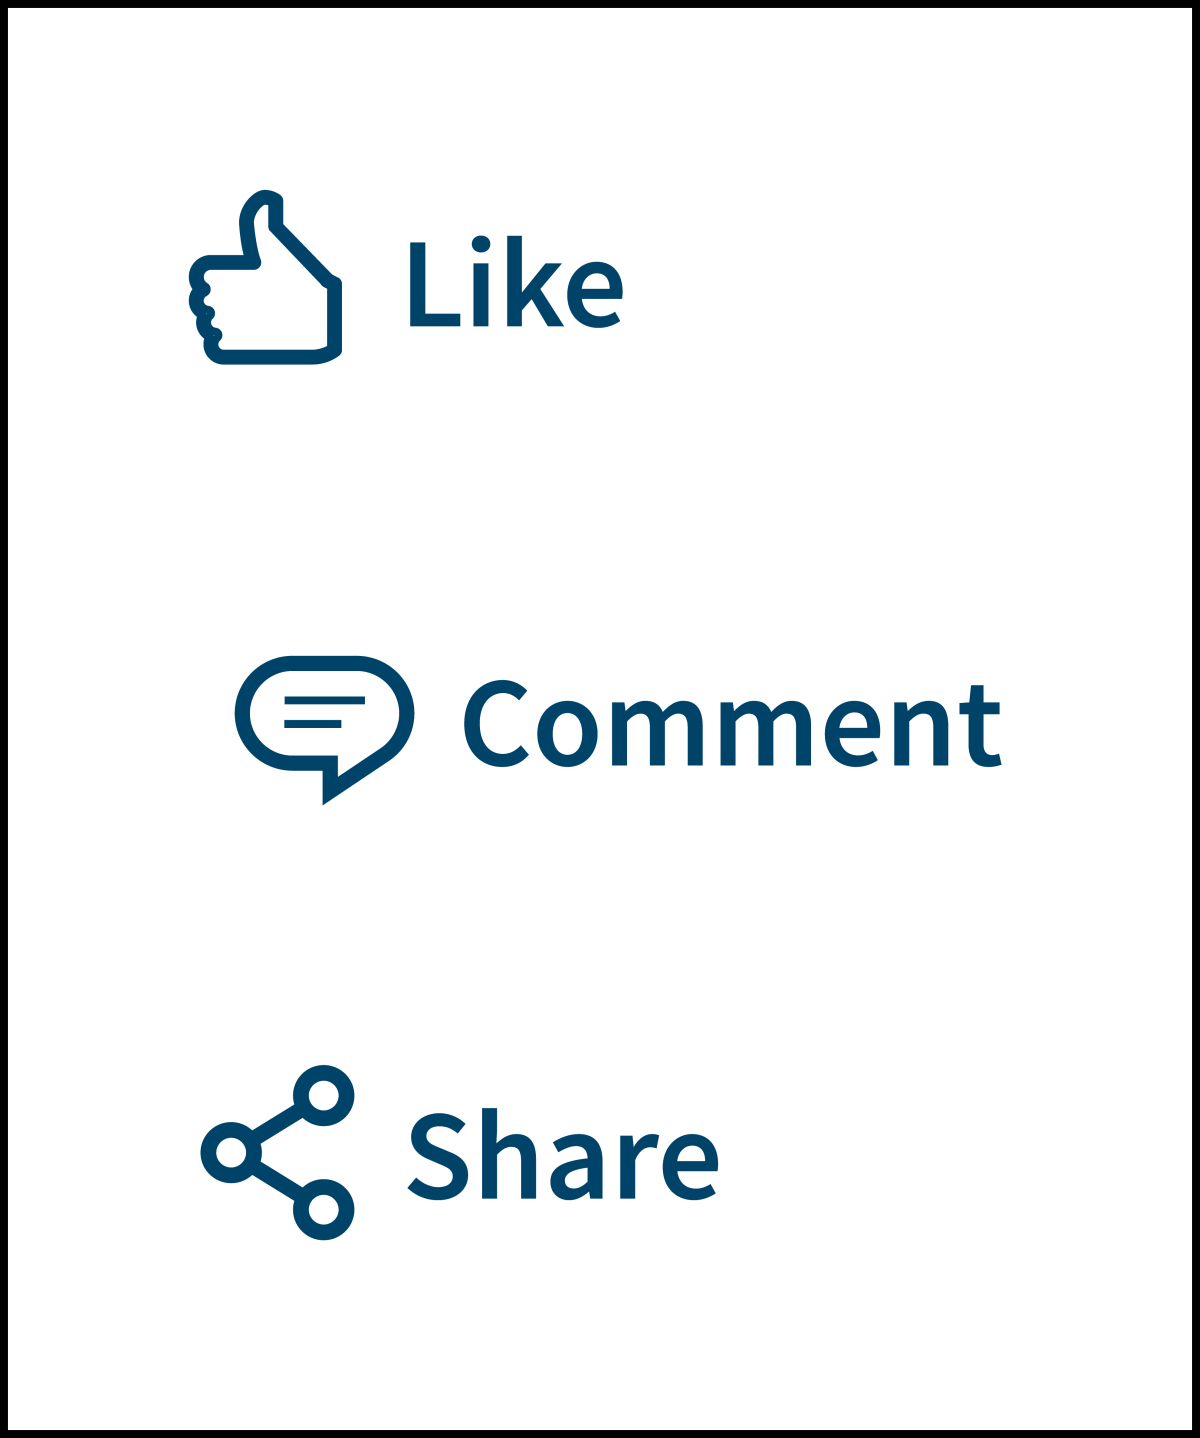
\includegraphics[width=0.5\textwidth]{Images/chapter_27/section_6676498603048960/4565554812944384.png}
\end{minipage}

% \vspace{-1.0\baselineskip}
\noindent
\begin{minipage}[t]{0.48\textwidth}\vspace{0pt}
\textbf{R10:} The system should notify the user about messages, connection requests, search appearances, or comments on their posts.
\\
\textbf{R11:} Users should be able to create company pages and follow other company pages.
\\
\textbf{R12:} Company pages can list job openings that users can apply for.
\\
\textbf{R13:} A user should be able to create and join groups.
\end{minipage}
\hfill
\begin{minipage}[t]{0.48\textwidth}\vspace{0pt}
\centering
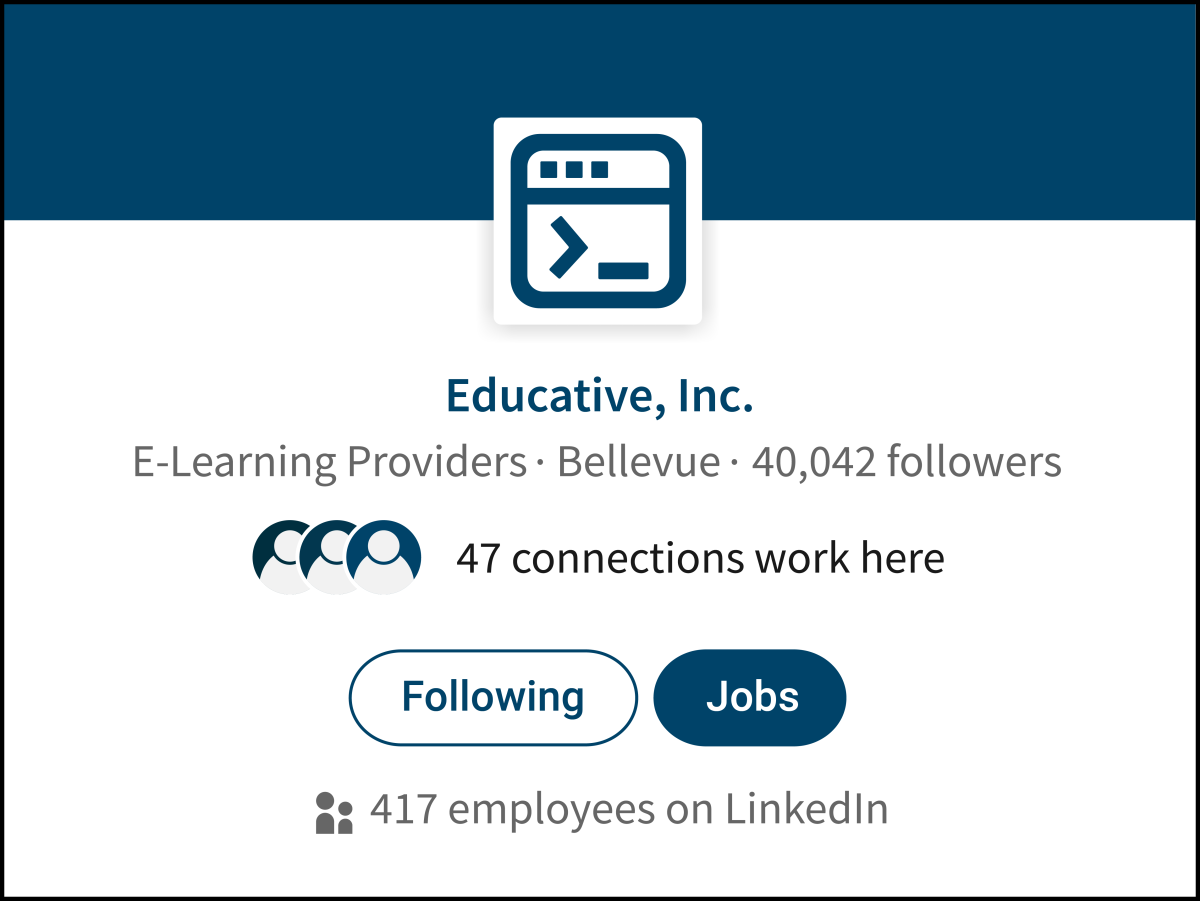
\includegraphics[width=0.5\textwidth]{Images/chapter_27/section_6676498603048960/4829158179078144.png}
\end{minipage}

We've identified our requirements for the problem. In the next lesson, we will define different use cases of LinkedIn.

% End of section content